\section{Study 3: Password Selection and Coping}
% ALINE
% GOALS
As a final step in our ``password personality'' exploration, we ran another online study. Having investigated policies and the perception of passwords through the lens of personality traits, the main goal of the third study was to evaluate potential associations between personality and password \textit{selection}. To overcome some of the limitations of the previous study, we hoped to increase the sample size and reduce the number of items during the study. Moreover, further answers about the participants' explanations and motivations were considered to better understand the weight of personality factors. We determined the following research questions: 1) Are there correlations between password features (topology) and personality traits? 2) Do certain facets of personality shine through in password coping strategies, e.g. the tendency to write down passwords?

\subsection{Procedure and Tools}
The study was designed to take no more than ten minutes. The briefing page informed participants about the purpose of the study and data disclosure policies. After acknowledging the conditions of participation, respondents were asked to create a password. To boost ecological validity, we provided a fictitious but realistic scenario \cite{Komanduri2011OfPasswordsAndPeople}. The task was to come up with a new password for a new email account that they were going to use as their main address. Further, the instruction pointed out that the incentive would only be paid of if the participants chose a password they could recall later on. A \textit{basic8} policy was enforced, as it is one of the most representative policies in the wild (see chapter \ref{chap:policies_reuse}). This loose policy would also allow for both very complex and rather simple passwords, which could be associated with personality traits. Having successfully confirmed the password, respondents were taken to a questionnaire about demographics, just like in the first two studies. 

Next, participants completed the BFI-K questionnaire consisting of 21 items that have to be rated on a 5-point scale. We opted not to use the 50-item inventory for the sake of saving time. We added an item that served as an attention check. It asked to respond to this item with ``disagree''. Failure to follow this instruction allowed us to drop the response from the dataset. The resulting 22 items were shuffled to avoid sequence effects. 

Afterwards, we surveyed respondents about their password management behaviors and preferences. We used multiple-choice and open responses to collect qualitative, self-reported data. For instance, we wanted to know how they cope with multiple accounts or how they reuse passwords. The survey concluded with a recall task, where participants provided their initially chosen password. They could try as often as they liked, and the number of attempts were recorded. In case they were unable to recall their password, they could proceed anyhow and take part in the lottery. If they chose to provide an email address in the final step, this data was stored separately from the questionnaire data to avoid privacy issues. 

\subsection{Recruitment and Sample}
Participants were invited via a university newsletter, and snowballing the link via personal connections and posts on social networks. The questionnaire was in German and participants were screened about their command of the German language. We instructed participants to take the survey on a desktop. 
%TODO aline says 184 but the data set is smaller :-/ ?
%all the following numbers are from the smaller data set.
184 people completed the survey, but we had to drop the responses of 8 participants because their response timings were unrealistically fast (lower than 2 * standard deviation). From the 176 remaining respondents, 89 were male, 86 female and 1 preferred not to answer. 116 were students, i.e. a rather high proportion (66\%). Consequently, the average age was 25 years (range [16;55], $SD$=6, $Md$= 24). 67 (38\%) reportedly had an IT-background. 129 respondents chose to participate in the raffle for shopping vouchers. 

\subsection{Limitations}
As many password-selection studies, our study is limited by the purposefulness of the task: Participants knew they were only going to use the password in the study. To mitigate this, we tried to give participants enough context information to immerse themselves into the situation. Moreover, while the study was ongoing, we received 30 feedback emails asking for clarification about the attention check questions. We had introduced an additional item at a random position in the personality construct. This led to misunderstandings that we failed to identify in the design and piloting of the survey. Some respondents thought that this question was a measure of their personality, too, and indicated giving a wrong answer on purpose. We therefore had to omit this sanity check entirely, because it did not feasibly tell whether participants had read the questions carefully enough. Instead, we based the decisions to drop responses on the timings. 

\subsection{Results}
% descriptives
The resulting passwords had a median-length of 10 characters ([8;22]) -- 130 participants went beyond the minimum requirement of eight characters. Figure \ref{fig:personality:study3:metrics-overview} visualizes additional metrics that show that passwords were also stronger than expected with a mean guess number greater than $10^8$. Passwords with guess numbers greater than $10^6$ are expected to withstand online attacks \cite{Florencio2014AdministratorsGuide}. Moreover, overall internal consistency of the big-five construct was at $\alpha=0.65$, thus slightly below the bar at 0.7. Subscales for each trait, however, were more consistent and above the threshold. In the following, we try to fit generalized additive models to the data using B5 trait scores as covariates. 
%TODO we could talk about more LUDS statistics

\begin{figure}[tbph]
	\centering
	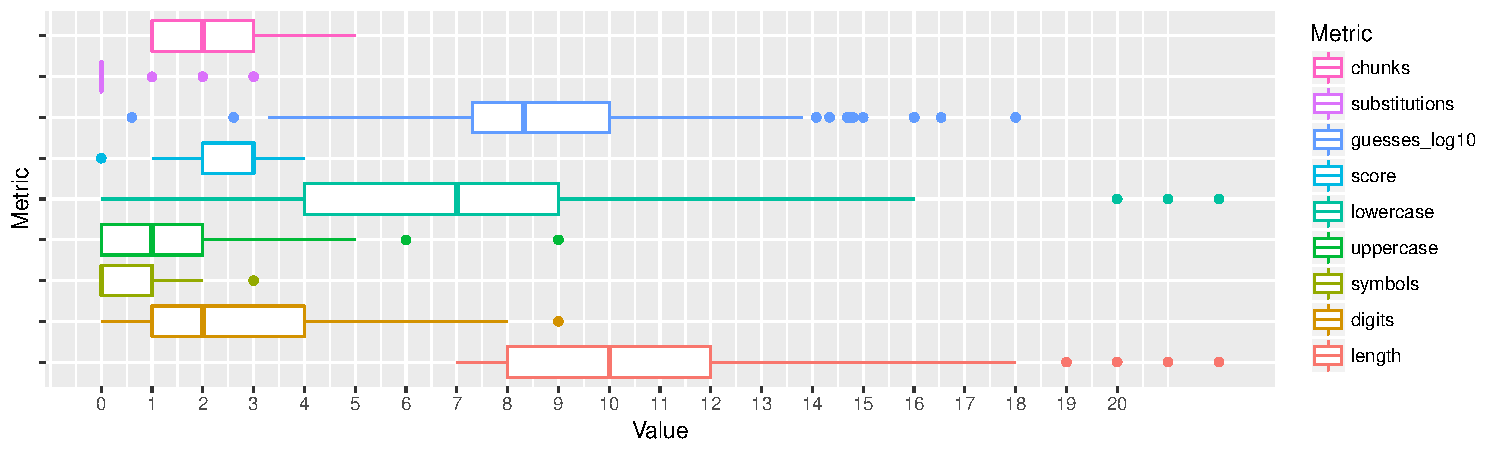
\includegraphics[width=1\linewidth]{figures/personality/study3-metrics-overview}
	\caption{\label{fig:personality:study3:metrics-overview} Zxcvbn metrics for user selected passwords.}
\end{figure}

% maximum R-sq 
\subsubsection{Password Composition}
%TODO aline's data suggests that all this was associated with agreeableness, instead of neuroticism, but I found a labelling error. discuss!
First, we use zxcvbn metrics as response variables, and explore marginal associations with big five traits. As before, we include age, gender and IT-background as control covariates. We found that only password length was (significantly) associated with B5-traits: Participants with higher \textit{neuroticism} scores tended to create longer passwords ($\beta = 0.21$), using more lower-case letters as a side effect ($\beta = 0.19$). A second corollary was that passwords from those participants also consisted of more word-chunks ($\beta= 0.26$). However, it is hard to read this result, because even very long random passwords consist of only one matching sequence (``bruteforce''), so more chunks does not imply greater strength. 
%control variables and model fit. 
Moreover, having an IT background was positively associated with password length ($\beta = 0.21$). A one-tailed Mann-Whitney test confirms this ($W=4204$,\pvallt{0.05}). Consequently, password guess numbers were higher if participants had an IT background ($\beta=0.19$). None of the models however, achieved exceptionally good fit: the maximum R-squared (adjusted) value was \Rsqadj{0.13} (for the number of symbols as target variable). We tried to achieve a better fit by performing a principal component and factor analyses. This was not effective, either. We conclude that password metrics are only very slightly predictable by personality profiles. 
%OPTIONAL point much smaller R-sq than in second study. 

%\subsection{Selection Strategies} -- no noteworthy association so we leave this out. and also I don't understand how Aline approached this. the categories seem too arbitrary. 

\subsubsection{Password Management Strategies}
Respondents freely reported reusing passwords (88.4\%), and 65.34\% said to categorize their passwords. Memorizing passwords was the preferred strategy for 109 participants, followed by notes on paper or a file ($n=43$). Using a password manager was generally the least favored option ($n=24$).

% binary -- logit model ``write down'': yes no
We created generalized additive logit models for every management strategy, i.e. binary outcomes like ``Using a password manager'': 1 (true) or 0 (false). Since the percentage of participants reusing passwords is so high, influence by personality traits was unlikely to be detected. Consequently, none of the associations was flagged as significant for reuse. However, older participants were more likely to reuse passwords as shown in Figure \ref{fig:personality:study3:age-openness-coping-all}. Extroverted participants were significantly less likely to write passwords down on paper or into a digital file ($\beta=-1.54$). Participants with an IT background showed fewer signs of password reuse ($\beta=-1.97$). Instead, they more likely used a password manager ($\beta=2.1$). Since having an IT background was significantly correlated with being male ($\chi^2=14.32, p < 0.001$), males were also more inclined to use a \gls{PWM}. We can observe another interesting aspect in Figure \ref{fig:personality:study3:age-openness-coping-all} which depicts associations between all tested coping strategies and openness scores, respectively age. Age and openness show an \textit{inverse} tendency towards using a password manager: while older participants seem to be more likely to use a \gls{PWM} ($\beta=0.77$), the opposite is the case for participants with higher openness scores ($\beta=-2.06$). Similarly, memorizing passwords was less likely for older, but more likely for ``open'' participants. Generally, memorizing passwords seems to be the \textbf{only} unfavorable coping strategy for older participants. 
\begin{figure}[tbph]
	\centering
	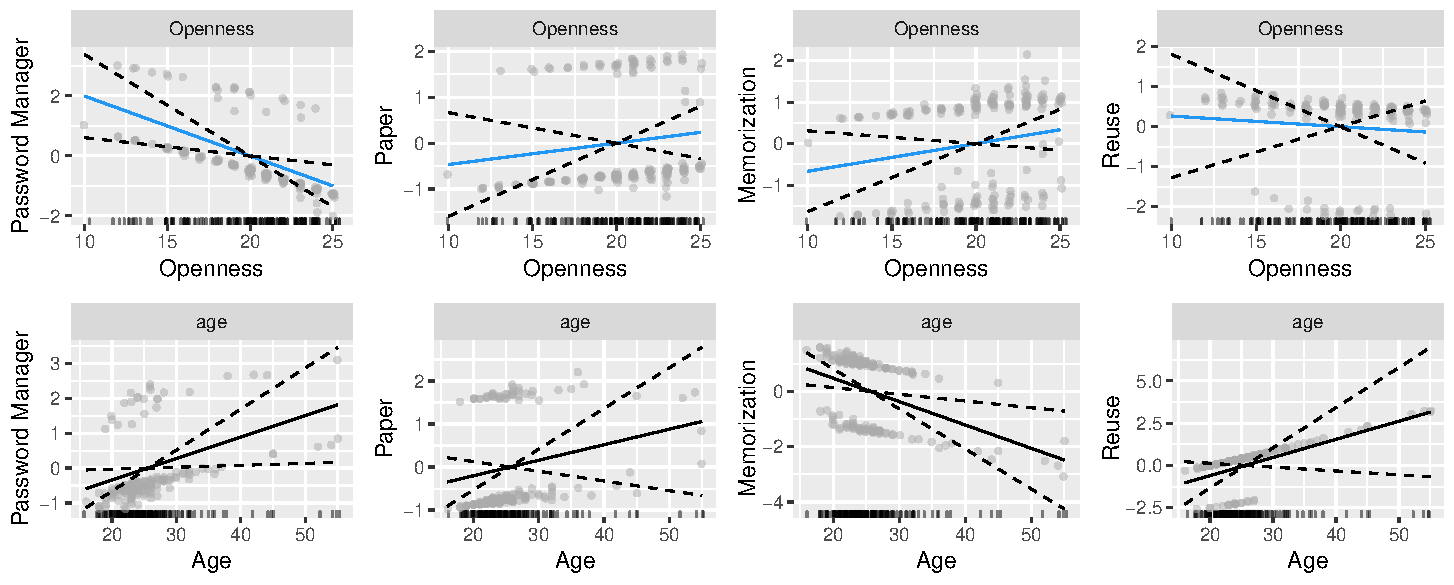
\includegraphics[width=1\linewidth]{figures/personality/age-openness-coping-all}
	\caption{\label{fig:personality:study3:age-openness-coping-all}Age and Openness model plots for all coping tested coping strategies. Openness and Age show inverse associations regarding password managers and memorization.}
\end{figure}

\subsubsection{Memorability}
Only 18 out of 176 participants (10\%) failed to recall the newly created password at the end of the survey. Thus, associations with personality traits were unlikely. However, it was clear even with only 18 passwords being forgotten that the length of the password significantly contributed to failure rates ($\beta=2.25$, \Rsqadj{0.19}, 25\% of explained deviance). The R-squared value drops significantly if we remove the Big-Five traits as predictors (\Rsqadj{0.07}, 8\% of explained deviance, \pvallt{0.05}). Thus, password memorability was associated with personality, but we are not able to tell exactly in which way. 

%\subsubsection{Other findings}
%One participant (P48) claimed that their password (\texttt{!Q\"W3e4}) was not based on keyboard patterns. Zxcvbn also failed to recognize the pattern, because it only is obvious on a keyboard with a German layout where the quotation marks are entered with Shift+2.
%Internal consistency analysis with the alpha function suggested to reverse neuroticism items to increase reliability. This is an odd finding, but could be due to chance. 

\subsection{Summary and Interpretation}
We observed that password length was marginally associated with Neuroticism, but no other personality traits. Higher neuroticism scores can be paraphrases as smaller emotional stability. Losing access to an account might lead to stronger emotional reactions. So, possibly, participants showing this trait want to make sure that this scenario does not happen by choosing a longer and stronger password. Participants working in or studying an IT-related field, were also more likely to pick longer passwords, but achieved significantly higher guess numbers. This corroborates findings from Mazurek \etal conclusively \cite{Mazurek2013Measuring}. Fitting generalized additive models to data of 176 participants did not show sufficiently strong model fits to warrant definite inferences about the influence of personality traits on password metrics. To a higher degree of certainty, however, we can state that personality must not be ruled out for password selection, which is an unprecedented result. We especially saw this when we dropped the big five scores as predictors for memorizing the password. 

Regarding the retrospective data, we did find salience. Although the overall sample shows that using a password manager is unattractive, a deeper analysis revealed that the participants' age and openness scores are linked to using a \gls{PWM}, or to memorization efforts. These predictors were inversely associated, which means that there could be a ``sweet spot'' of openness scores and age. Consequently, this gives us the opportunity to segment target groups for password managers more effectively: Older users might be more receptive for password support tools. Lower openness scores indicate that people are more conservative, ``down to earth'', and appreciate conventions \cite{McCrae1987ValidationFFM}. These values also appear plausible for older participants in the light of related research \cite{Srivastava2003PersonalityAdulthood}. Thus, we conclude that the design of future password support tools should be centered on different age groups. We will also see in Chapters \ref{chap:mental_models_pwm} and \ref{chap:pwrm} that none of the current solutions is specifically tailored to different user groups. Current one-size-fits-all solutions might hence explain to some degree why \glspl{PWM} are still underused.


%TODO binary outcome (memorability) needs a larger sample to pinpoint the marginal associations of personality traits with memorability. 